%%% LaTeX Template: Article/Thesis/etc. with colored headings and special fonts
%%%
%%% Source: http://www.howtotex.com/
%%% Feel free to distribute this template, but please keep to referal to http://www.howtotex.com/ here.
%%% February 2011
%%%
%%% Modified January 2016 by CDM

%%%  Preamble
\documentclass[11pt,letterpaper]{article}
\usepackage[margin=1.0in]{geometry}
\usepackage[T1]{fontenc}
\usepackage[bitstream-charter]{mathdesign}
\usepackage[latin1]{inputenc}					
\usepackage{amsmath}						
\usepackage{xcolor}
\usepackage{cite}
\usepackage{hyphenat}
\usepackage{graphicx}
\usepackage{float}
\usepackage{subfigure}
\usepackage{sectsty}
\usepackage[compact]{titlesec} 
\usepackage[tablegrid]{vhistory}
\usepackage{pbox}
\allsectionsfont{\color{accentcolor}\scshape\selectfont}

%%% Definitions
\definecolor{accentcolor}{rgb}{0.0,0.0,0.5} 
\newcommand{\teamname}{TrafficNetPeons}
\newcommand{\productname}{Product Name: TBD}
\newcommand{\coursename}{CSE 4316: Senior Design I}
\newcommand{\semester}{Spring 2016}
\newcommand{\docname}{Architectural Design Specification}
\newcommand{\department}{Department of Computer Science \& Engineering}
\newcommand{\university}{The University of Texas at Arlington}
\newcommand{\authors}{Peyton Casper \\ Rabin Dhaubonjar \\ Kyle Edelmann \\ Jose Hernandez \\ Ruchitha Thalakola}

%%% Headers and footers
\usepackage{fancyhdr}
	\pagestyle{fancy}						% Enabling the custom headers/footers
\usepackage{lastpage}	
	% Header (empty)
	\lhead{}
	\chead{}
	\rhead{}
	% Footer
	\lfoot{\footnotesize \teamname \ - \semester}
	\cfoot{}
	\rfoot{\footnotesize page \thepage\ of \pageref{LastPage}}	% "Page 1 of 2"
	\renewcommand{\headrulewidth}{0.0pt}
	\renewcommand{\footrulewidth}{0.4pt}

%%% Change the abstract environment
\usepackage[runin]{abstract}			% runin option for a run-in title
%\setlength\absleftindent{30pt}			% left margin
%\setlength\absrightindent{30pt}		% right margin
\abslabeldelim{\quad}	
\setlength{\abstitleskip}{-10pt}
\renewcommand{\abstractname}{}
\renewcommand{\abstracttextfont}{\color{accentcolor} \small \slshape}	% slanted text

%%% Start of the document
\begin{document}

%%% Cover sheet
{\centering \huge \color{accentcolor} \sc \textbf{\department \\ \university} \par}
\vspace{1 in}
{\centering \huge \color{accentcolor} \sc \textbf{\docname \\ \coursename \\ \semester} \par}
\vspace{0.5 in}
\begin{figure}[h!]
	\centering
   	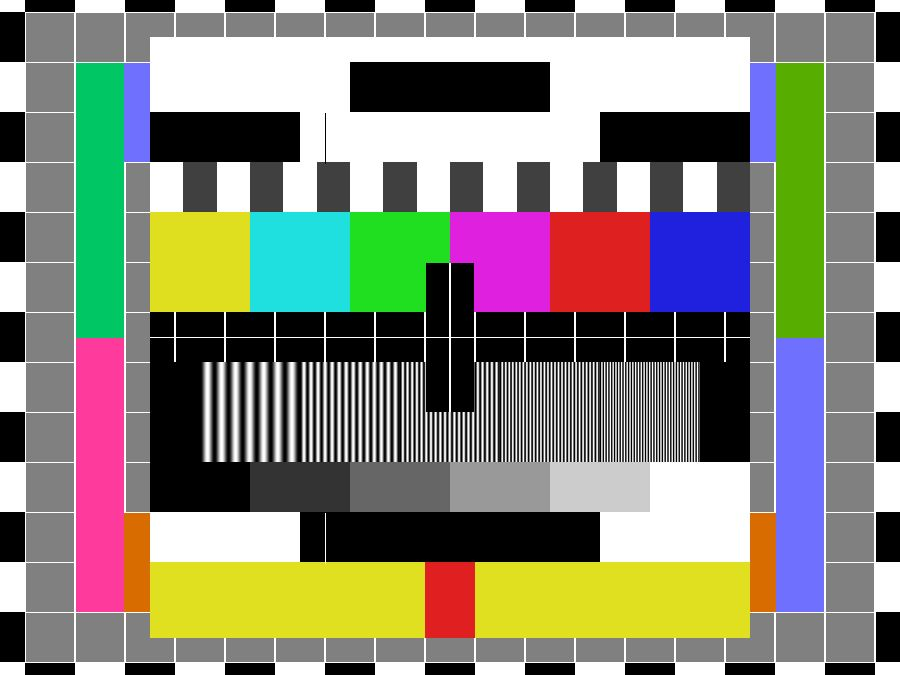
\includegraphics[width=0.60\textwidth]{images/test_image}
\end{figure}
\vspace{0.5 in}
{\centering \huge \color{accentcolor} \sc \textbf{\teamname \\ \productname} \par}
\vspace{0.5 in}
{\centering \large \sc \textbf{\authors} \par}
\newpage


%\vspace{1 in}
%\centerline{January 13th, 2012}
%\newpage

%%% Revision History
\begin{versionhistory}
  	\vhEntry{0.1}{04.01.2016}{PC}{Document Creation}
  	\vhEntry{0.2}{04.06.2016}{PC|JH|RT|RD|KE}{Initial Draft Complete}
  	\vhEntry{0.3}{04.07.2016}{PC|JH|RT|RD|KE}{Updated Draft}
  	\vhEntry{1.0}{04.08.2016}{PC|JH|RT|RD|KE}{Document Release}
\end{versionhistory}
\newpage

%%% Table of contents
\setcounter{tocdepth}{2}
\tableofcontents
\newpage

%%% List of figures and tables (optional)
\listoffigures
\listoftables
\newpage

%%% Document sections
\section{Introduction}
Your introduction should describe your product concept in sufficient detail that the architectural design will be easy to follow. The introduction may include information used in the first sections of your SRS for this purpose. At a minimum, ensure that the product concept, scope and key requirements are described.
\newpage
\section{System Overview}
In our system there are four main layers, which are classified as web interface layer, wireless connection layer, base station layer, camera layer. The user can communicate with the remote surveillance camera with the help of the user interface. The Ethernet and black box will bridge between the user and the remote camera. User interface will include all kinds of resources that user is capable of using. In the system streaming video is made available and some of the controls that user can use through his computer. In the camera layer we have our camera module, which can be rotated and tilted 180 degrees, which makes it 360- degree total movement possible. In the network layer we will be using Ethernet connection. The source of the power for the camera layer and black box is base station. The main power source for the base station is solar battery.



\begin{figure}[h!]
	\centering
 	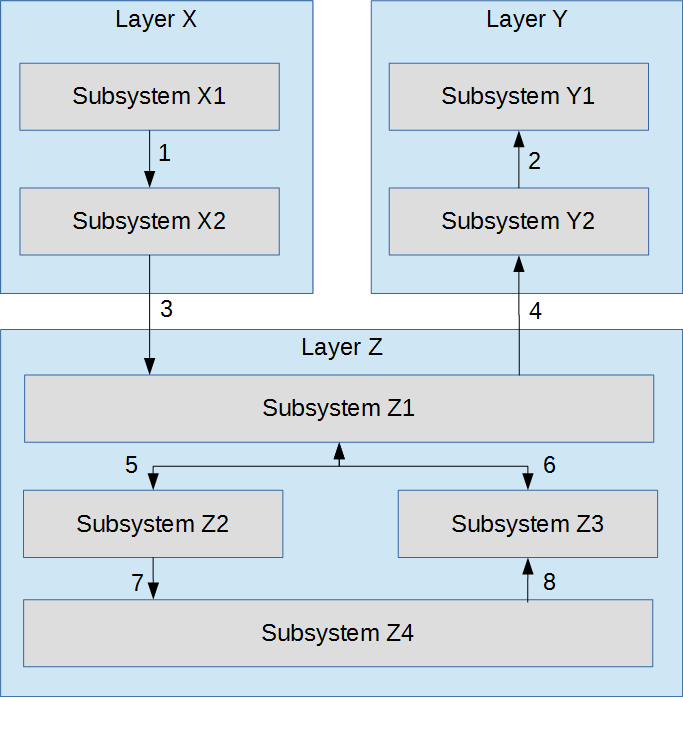
\includegraphics[width=0.90\textwidth]{images/data_flow}
 \caption{System architecture}
\end{figure}

\newpage
\section{Subsystem Definitions \& Data Flow}
In our camera system there are four different layer web interface layer, wireless connection layer, base station layer and camera layer. Each and every camera has their unique IP address. When the user selects the camera to view then the login screen will have popped up. User will be asked to put the valid username, password as well as IP address of the camera to get the access. When the user enters the username, password and IP address then the system will compare the data entered with the data saved in the raspberry pi. The data will be sent wirelessly, which is received by the black box connected to the raspberry pi through Ethernet connection. If the data entered is valid then the system will take the user to screen, which contains the live streaming video and arrow keys button, which user can use to control the movement of the camera. If the user wants to move the camera and press button, then the message will be sent and which be received by the black box then sent to the raspberry pi. The raspberry pi will control the movement of the stepper. To control the movement of the stepper motors arrow key will be used. At the same time base station will be set up on the remote location which will be main source of the power for the camera layer. As soon as user login, user can start viewing the live streaming video, which user does not have to request. The zoom in and zoom out functionality works in the same way as moving the camera module.


\begin{figure}[h!]
	\centering
 	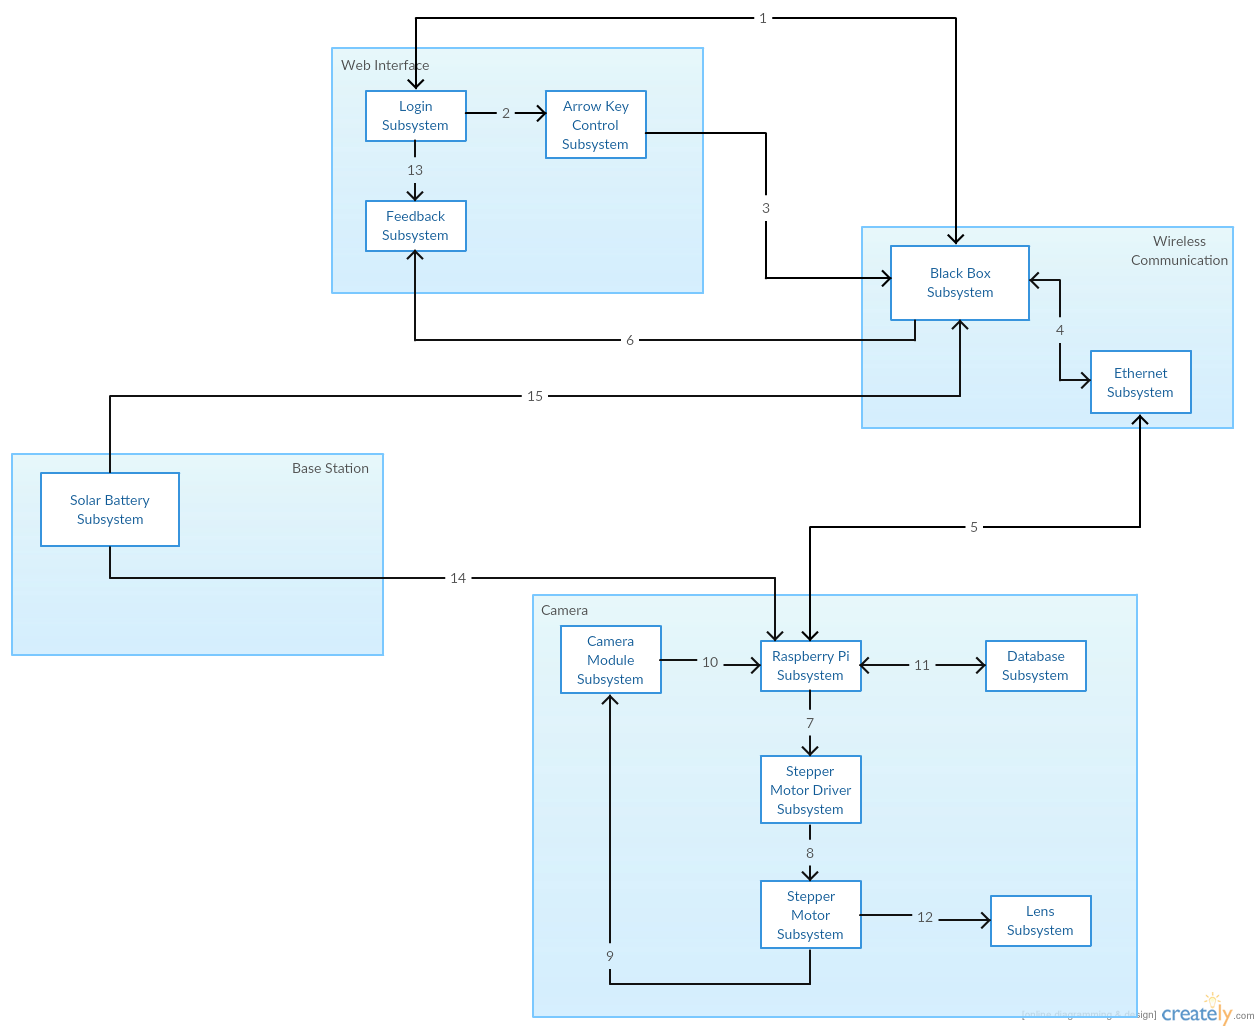
\includegraphics[width=\textwidth]{architectural design specification latex/images/ADSdiagrams/subsystem_definitions_and_dataflow.png}
 \caption{A simple data flow diagram}
\end{figure}

\newpage
\section{X Layer Subsystems}
The following sections are dedicated to the Wireless Communications Layer of this project. This layer includes the Ethernet Subsystem and the Black Box Subsystem. The Wireless Communications Layer manages the communications demands between the Web Interface Layer and the Camera Layer via UDP transport protocol over a wireless network provided the consumer by TrafficNet LLC.

\subsection{Black Box Subsystem}

\begin{figure}[h!]
	\centering
 	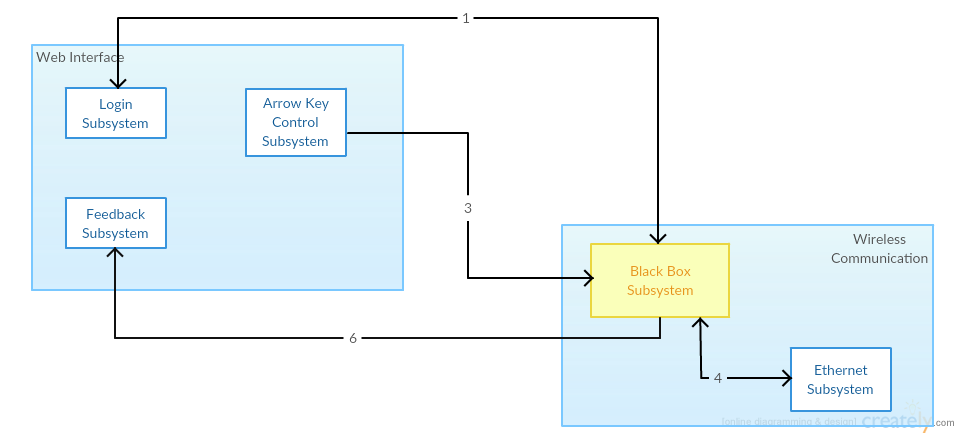
\includegraphics[width=0.60\textwidth]{images/ADS diagrams/blackboxsubsystem.png}
 \caption{Black Box description diagram}
\end{figure}

The above diagram illustrates graphically the interaction of the Black Box Subsystem with other Subsystems from the Web Interface Layer. 

\subsubsection{Assumptions}
The Black Box Subsystem is one of two Subsystems that is necessary for this Architectural Design Specification but is provided entirely by TrafficNet LLC. Therefore it is assumed to be the responsibility of the vendor to provide.

\subsubsection{Responsibilities}
The Black Box provides the secure wireless communication between the Web based UI and the Raspberry Pi housed within the Camera. ZeroMQ establishes a TCP transfer protocol over a wireless network provided by the Black Box that may be accessed only by authorized users from a directly linked host machine. Authorized users may then use this network to send control signals from the host machine through the wireless network to the Raspberry Pi, as well as receive video feedback through the wireless network provided by the Black Box.

\subsubsection{Subsystem Interfaces}

\begin {table}[H]
\caption {Subsystem interfaces} 
\begin{center}
    \begin{tabular}{ | p{1cm} | p{6cm} | p{3cm} | p{3cm} |}
    \hline
    ID & Description & Inputs & Outputs \\ \hline
    \#1, 3, 4, 6 & Interaction between Black Box and the Web Interface/bus & \pbox{3cm}{Login server \\ Arrow Key Control \\ Ethernet} & \pbox{3cm}{Video Feedback \\ Login validation \\ TCP segments}  \\ \hline
    \end{tabular}
\end{center}
\end{table}

\subsection{Ethernet Subsystem}

\begin{figure}[h!]
	\centering
 	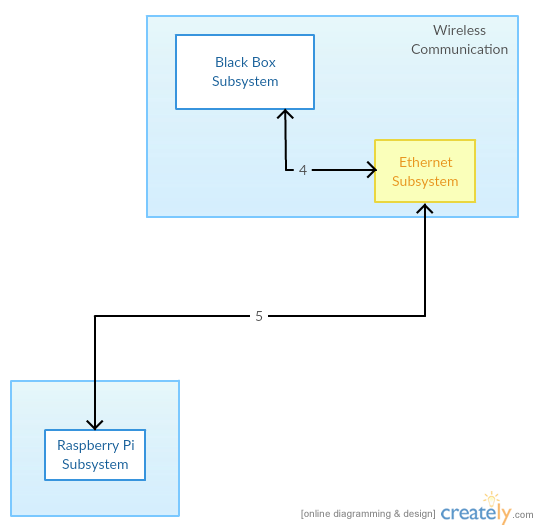
\includegraphics[width=0.60\textwidth]{images/ADS diagrams/ethernetsubsystem.png}
 \caption{Ethernet description diagram}
\end{figure}

The above diagram illustrates graphically the interaction between the Ethernet Subsystem, the Black Box Subsystem, and the Raspberry Pi Subsystem of the Camera Layer. 

\subsubsection{Assumptions}
The Ethernet Subsystem is the physical connection between the Black Box Subsystem and the Raspberry Pi Subsystem of the Camera Layer.

\subsubsection{Responsibilities}
The Ethernet Subsystem is responsible for providing a physical link between the Black Box provided by TrafficNet LLC and the Raspberry Pi. It is the point at which wireless commands are physically recieved by the Camera Layer from the Wireless Communications Layer, and sent in the form of video feedback through the wireless network.

\subsubsection{Subsystem Interfaces}

\begin {table}[H]
\caption {Subsystem interfaces} 
\begin{center}
    \begin{tabular}{ | p{1cm} | p{6cm} | p{3cm} | p{3cm} |}
    \hline
    ID & Description & Inputs & Outputs \\ \hline
    \#4, 5 & Interaction between Raspberry Pi and the Ethernet/bus & \pbox{3cm}{Black Box Wireless Commands \\ Raspberry Pi TCP Communication} & \pbox{3cm}{Video Feedback \\ Login validation \\ TCP segments}  \\ \hline
    \end{tabular}
\end{center}
\end{table}

\newpage
\section{Y Layer Subsystems}
The following sections are dedicated to the Camera Layer of this project. This layer includes Raspberry Pi 2, database, stepper motor drivers, stepper motor, lens, and camera module subsystems. The Camera Layer manages the actions set fourth by the user in the Web Interface layer.

\subsection{Raspberry Pi Subsystem}

\begin{figure}[h!]
	\centering
 	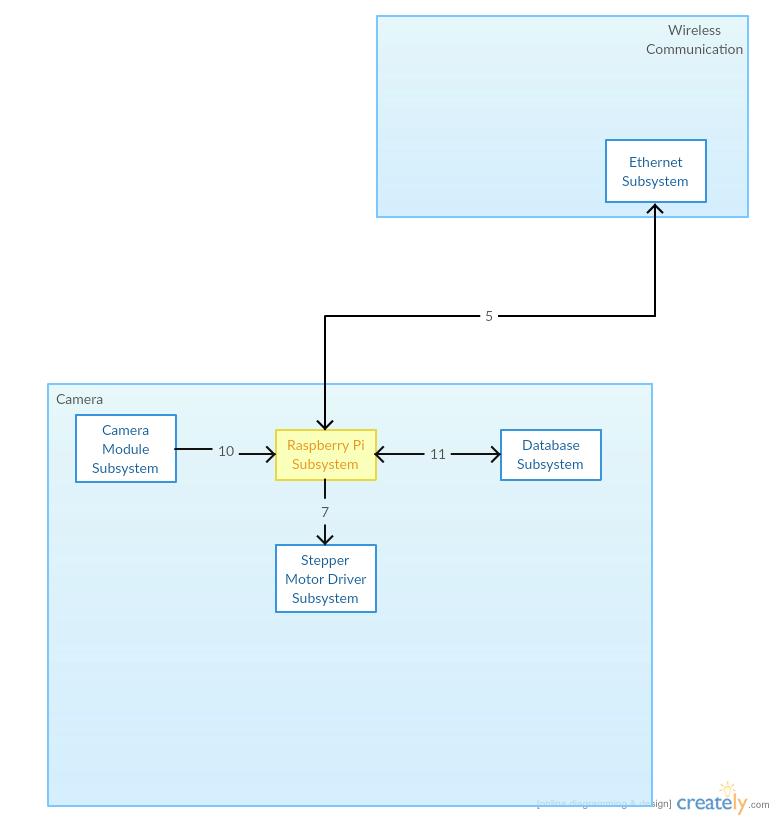
\includegraphics[width=0.60\textwidth]{images/ADS diagrams/raspberry_pi_subsystem.png}
 \caption{Raspberry Pi Subsystem Description}
\end{figure}

The above diagram illustrates graphically the interaction of the Raspberry Pi Subsystem with other Subsystems from the Camera Layer.

\subsubsection{Assumptions}
The camera layer is assumed to have Ethernet connection and web interface prior to controlling the camera and its movements. Stepper motor and camera module are physically hard wired to the Raspberry Pi. 

\subsubsection{Responsibilities}
The Raspberry Pi 2 is controlled by user input in the web interface layer, which is then responsible for controlling all other subsystems in the camera layer.

\subsubsection{Subsystem Interfaces}

\begin {table}[H]
\caption {Subsystem interfaces} 
\begin{center}
    \begin{tabular}{ | p{1cm} | p{6cm} | p{3cm} | p{3cm} |}
    \hline
    ID & Description & Inputs & Outputs \\ \hline
    \#5, 7, 10, 11 & Controls all other subsystems in the camera layer/bus & \pbox{3cm}{Ethernet \\ Module \\ Database } & \pbox{3cm}{Stepper motor drivers \\ Database}  \\ \hline
   
    
    \end{tabular}
\end{center}
\end{table}



\subsection{Database Subsystem}

\begin{figure}[h!]
	\centering
 	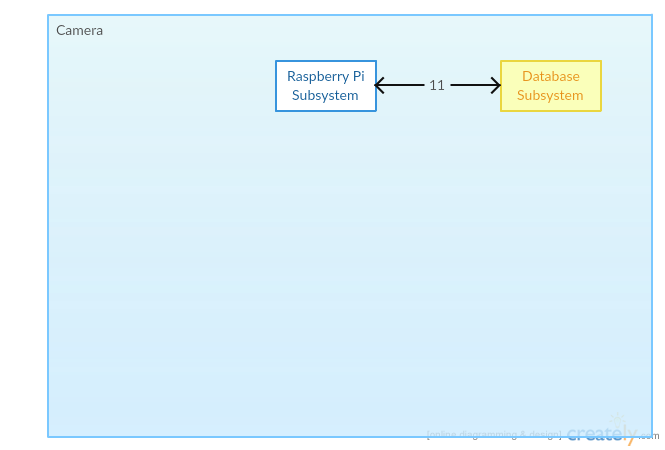
\includegraphics[width=0.60\textwidth]{images/ADS diagrams/database_subsystem.png}
 \caption{Database Subsystem Description}
\end{figure}

The above diagram illustrates graphically the interaction of the Database Subsystem with the Raspberry Pi Subsystem.

\subsubsection{Assumptions}
The camera layer is assumed to have Ethernet connection and web interface prior to controlling the camera and its movements.  

\subsubsection{Responsibilities}
The Rpi 2 has Ethernet connection, so all the information sent and received by the Raspberry Pi is stored in the database, which is used to store logs of important information.

\subsubsection{Subsystem Interfaces}

\begin {table}[H]
\caption {Subsystem interfaces} 
\begin{center}
    \begin{tabular}{ | p{1cm} | p{6cm} | p{3cm} | p{3cm} |}
    \hline
    ID & Description & Inputs & Outputs \\ \hline
    \#11 & Keep user interaction logs/bus & \pbox{3cm}{Raspberry Pi } & \pbox{3cm}{Raspberry Pi}  \\ \hline
   
    
    \end{tabular}
\end{center}
\end{table}






\subsection{Camera Module Subsystem}
\begin{figure}[h!]
	\centering
 	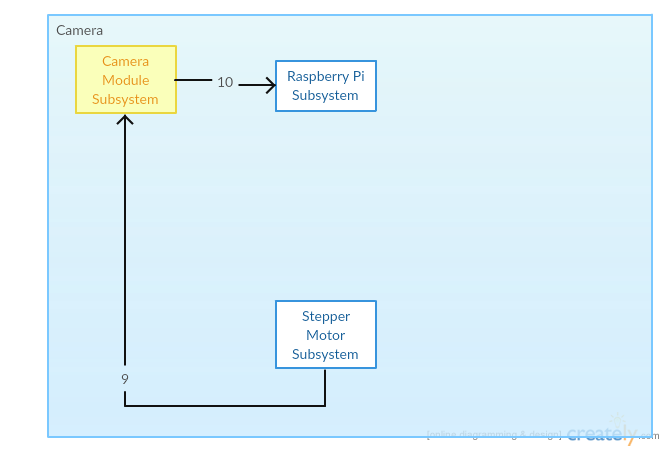
\includegraphics[width=0.60\textwidth]{images/ADS diagrams/camera_module_subsystem.png}
 \caption{Camera Module Subsystem Description}
\end{figure}

The above diagram illustrates graphically the interaction of the Camera Module Subsystem with the Raspberry Pi and Stepper Motor Subsystems.

\subsubsection{Assumptions}
The camera layer is assumed to have Ethernet connection and web interface prior to controlling the camera and its movements. The camera module is hard wired to the Raspberry Pi.  

\subsubsection{Responsibilities}
The lens is mounted to the camera module. The camera module is then controlled by the stepper motor, which moves the camera (pan and tilt) certain degrees based on user interactions. The camera module is responsible for capturing images of the surrounding landscape.

\subsubsection{Subsystem Interfaces}

\begin {table}[H]
\caption {Subsystem interfaces} 
\begin{center}
    \begin{tabular}{ | p{1cm} | p{6cm} | p{3cm} | p{3cm} |}
    \hline
    ID & Description & Inputs & Outputs \\ \hline
    \#10, 11 & Campture images/bus & \pbox{3cm}{Stepper motor } & \pbox{3cm}{Raspberry Pi}  \\ \hline
    
    
    \end{tabular}
\end{center}
\end{table}





\subsection{Lens Subsystem}
\begin{figure}[h!]
	\centering
 	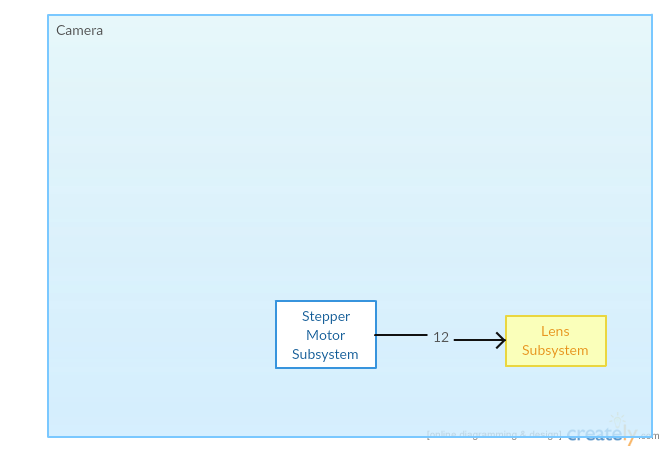
\includegraphics[width=0.60\textwidth]{images/ADS diagrams/lens_subsystem.png}
 \caption{Lens Subsystem Description}
\end{figure}

The above diagram illustrates graphically the interaction of the Lens Subsystem with the Stepper Motor Subsystem.

\subsubsection{Assumptions}
The camera layer is assumed to have Ethernet connection and web interface prior to controlling the camera and its movements. The lens is physically mounted on to the camera module.  

\subsubsection{Responsibilities}
The lens is responsible for providing camera quality images. The lens is mounted to the camera module. The camera module is then controlled by the stepper motor, which moves the camera (pan and tilt) certain degrees based on user interactions.

\subsubsection{Subsystem Interfaces}

\begin {table}[H]
\caption {Subsystem interfaces} 
\begin{center}
    \begin{tabular}{ | p{1cm} | p{6cm} | p{3cm} | p{3cm} |}
    \hline
    ID & Description & Inputs & Outputs \\ \hline
    \#12 & Improve camera quality images/bus & \pbox{3cm}{Stepper motor } & \pbox{3cm}{N/A}  \\ \hline
    
    
    \end{tabular}
\end{center}
\end{table}






\subsection{Stepper Motor Driver Subsystem}
\begin{figure}[h!]
	\centering
 	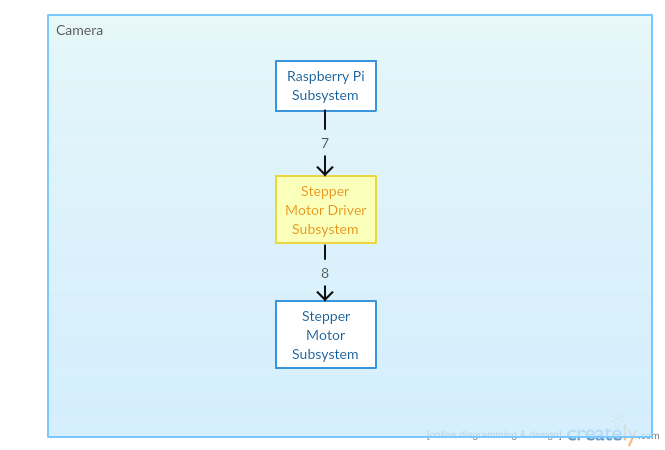
\includegraphics[width=0.60\textwidth]{images/ADS diagrams/stepper_motor_driver_subsystem.png}
 \caption{Stepper Motor Driver Subsystem Description}
\end{figure}

The above diagram illustrates graphically the interaction of the Stepper Motor Driver Subsystem with the Raspberry Pi and Stepper Motor Subsystems.

\subsubsection{Assumptions}
The camera layer is assumed to have Ethernet connection and web interface prior to controlling the camera and its movements.  

\subsubsection{Responsibilities}
The stepper motor driver is essentially software installed on the Raspberry Pi to control the stepper motors and allow the stepper motors to work.

\subsubsection{Subsystem Interfaces}

\begin {table}[H]
\caption {Subsystem interfaces} 
\begin{center}
    \begin{tabular}{ | p{1cm} | p{6cm} | p{3cm} | p{3cm} |}
    \hline
    ID & Description & Inputs & Outputs \\ \hline
    \#7, 8 & Allow stepper motors to work/bus & \pbox{3cm}{Raspberry Pi } & \pbox{3cm}{Stepper Motor}  \\ \hline
   
    
    \end{tabular}
\end{center}
\end{table}






\subsection{Stepper Motor Subsystem}
\begin{figure}[h!]
	\centering
 	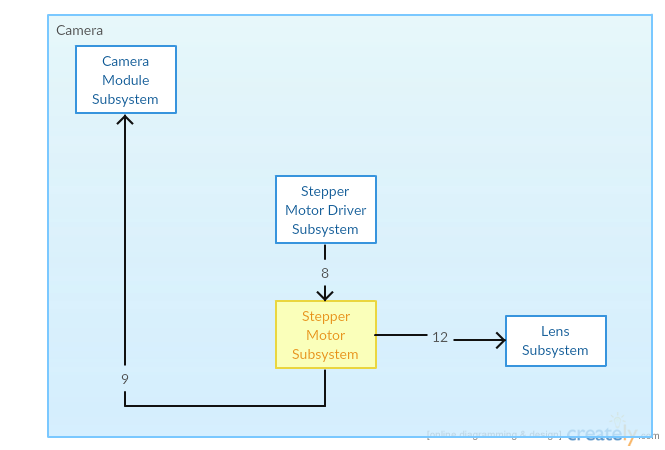
\includegraphics[width=0.60\textwidth]{images/ADS diagrams/stepper_motor_subsystem.png}
 \caption{Stepper Motor Subsystem Description}
\end{figure}

The above diagram illustrates graphically the interaction of the Stepper Motor Subsystem with the Stepper Motor Driver, Lens, and Camera Module Subsystems.

\subsubsection{Assumptions}
The camera layer is assumed to have Ethernet connection and web interface prior to controlling the camera and its movements. The Stepper Motor is physically hard wired to the Raspberry Pi. 

\subsubsection{Responsibilities}
The stepper motor driver is essentially software installed on the Rpi2 to control the stepper motors. The stepper motors are connected to the GPIO in the Rpi2 through wires. The lens is responsible for improving camera quality images. The lens is mounted to the stepper motor which moves based on user interaction. The camera module is also controlled by the stepper motor, which moves the camera (pan and tilt) certain degrees based on user interactions.

\subsubsection{Subsystem Interfaces}

\begin {table}[H]
\caption {Subsystem interfaces} 
\begin{center}
    \begin{tabular}{ | p{1cm} | p{6cm} | p{3cm} | p{3cm} |}
    \hline
    ID & Description & Inputs & Outputs \\ \hline
    \#8, 9, 12 & Control lens and camera module/bus & \pbox{3cm}{Stepper motor driver} & \pbox{3cm}{Lens \\ Camera Module}  \\ \hline
   
    \end{tabular}
\end{center}
\end{table}


\newpage
\section{Z Layer Subsystems}
This section details the web interface layer and the three subsystems that it encompasses. The web interface layer includes the login, feedback and arrow key interface subsystems.


In this section, the layer is described in some detail in terms of its specific subsystems. Describe each of the layers and its subsystems in a separate chapter/major subsection of this document. The content of each subsystem description should be similar. Include in this section any special considerations and/or trade-offs considered for the approach you have chosen.

\subsection{Login Subsystem}
The login sybststen will receive internet access from the black box system and be the first interface that the user will arrive at. The user will be required to access the system using a password or username stored in a database on the Raspberry Pi.

\begin{figure}[h!]
	\centering
 	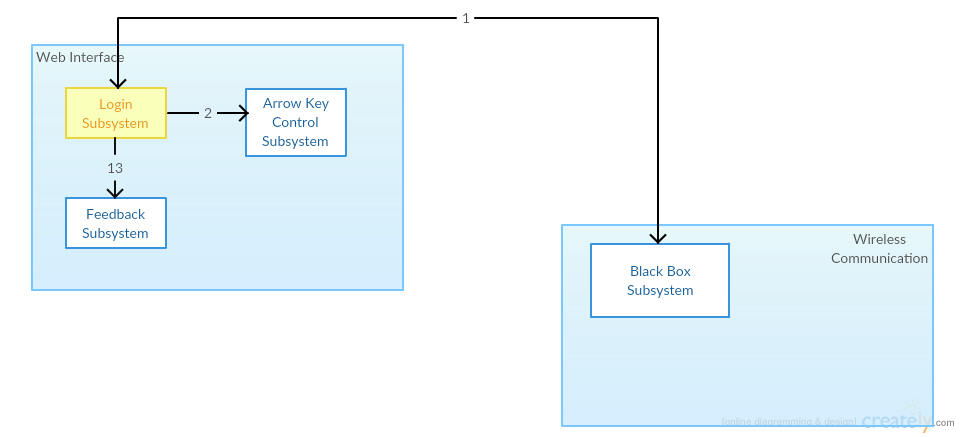
\includegraphics[width=0.60\textwidth]{images/ADSdiagrams/login_subsystem.png}
 \caption{Diagram of the Login Subsystem}
\end{figure}

\subsubsection{Assumptions}
The login subsystem relies on an internet connection to allow users to connect to it and access the camera feed.

\subsubsection{Responsibilities}
Each of the responsibilities/features/functions/services of the subsystem as identified in the architectural summary must be expanded to more detailed responsibilities. These responsibilities form the basis for the identification of the finer-grained responsibilities of the layer's internal subsystems. Clearly describe what each subsystem does.

\subsubsection{Login Subsystem  Interfaces}

\begin {table}[H]
\caption {Login Subsystem Interfaces} 
\begin{center}
    \begin{tabular}{ | p{1cm} | p{6cm} | p{3cm} | p{3cm} |}
    \hline
    ID & Description & Inputs & Outputs \\ \hline
    \#1 & The interface between the blackbox and the login system provides an internet connection so the user can communicate with the web interface.  & \pbox{3cm}{Incoming internet connection and the user's username and password} & \pbox{3cm}{Validation or rejection of the username and a redirection to the cameras feed if successful}  \\ \hline
    \#2 & This interface is reached after a successful validaion from the login system. & \pbox{3cm}{N/A} & \pbox{3cm}{The login system redirects the user to the Arrow Key Control Subsystem}  \\ \hline
    \#13 & The login system redirects to the feedback system on successful validaion. & \pbox{3cm}{N/A} & \pbox{3cm}{Validation of user login and redirect to }  \\ \hline	
    \end{tabular}
\end{center}
\end{table}


\subsection{Arrow Key Control Subsystem}
The arrow key control subsystem is reached after a successful validation from the login subsystem and provides the ability to pan and tilt the camera.

\begin{figure}[h!]
	\centering
 	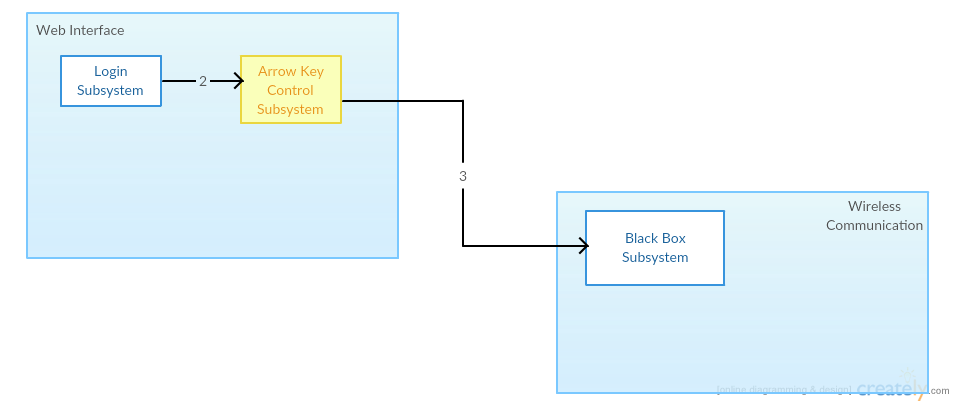
\includegraphics[width=0.60\textwidth]{images/ADSdiagrams/arrow_key_control_subsystem.png}
 \caption{Diagram of the arrow key control subsystem}
\end{figure}

\subsubsection{Assumptions}
The arrow key control subsystem assumes the user has been validated by the login subsystem.

\subsubsection{Responsibilities}
The arrow key control subsystem is responsible for ensuring that the user is able to control the camera's pan and tilt functionality, which includes relaying commands to the respective stepper motors.

\subsubsection{Arrow Key Control Subsystem Interfaces}

\begin {table}[H]
\caption {Arrow Key Control Interfaces} 
\begin{center}
    \begin{tabular}{ | p{1cm} | p{6cm} | p{3cm} | p{3cm} |}
    \hline
    ID & Description & Inputs & Outputs \\ \hline
    \#2 & This interface is reached after a successful validaion from the login system. & \pbox{3cm}{Successful validation and a redirect to the arrow key control subsystem} & \pbox{3cm}{N/A}  \\ \hline
    \#3 & The interface between the blackbox and the arrow key control subsystem provides an internet connection so the user can communicate with the web interface.  & \pbox{3cm}{N/A} & \pbox{3cm}{Control of the camera's stepper motors and verification to the user that the camera responded via the blackbox subsystem.}  \\ \hline

    \end{tabular}
\end{center}
\end{table}


\subsection{Feedback Subsystem Subsystem}
The feedback subsystem is responsible for relaying the camera feed back to the user once they have been successfully validated by the login subsystem.

\begin{figure}[h!]
	\centering
 	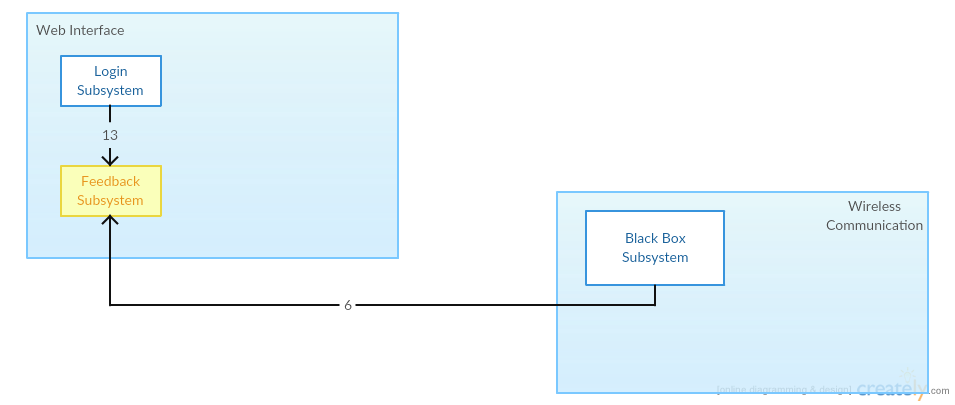
\includegraphics[width=0.60\textwidth]{images/ADSdiagrams/feedback_subsystem.png}
 \caption{Diagram of the feedback subsystem}
\end{figure}

\subsubsection{Assumptions}
The feedback subsystem assumes the user has been validated by the login subsystem and that the camera is operational.

\subsubsection{Responsibilities}
The feedback subsystem is responsible for fetching the current image from the camera and relaying that information back to the user.

\subsubsection{Feedback Subsystem Interfaces}

\begin {table}[H]
\caption {Feedback Interfaces} 
\begin{center}
    \begin{tabular}{ | p{1cm} | p{6cm} | p{3cm} | p{3cm} |}
    \hline
    ID & Description & Inputs & Outputs \\ \hline
 \#13 & The interface between the blackbox and the feedback subsystem provides an internet connection so the feedback subsystem can send back the requested image to the user.  & \pbox{3cm}{N/A} & \pbox{3cm}{The request image feed of the camera.}  \\ \hline
    \#13 & This interface is reached after a successful validaion from the login system. & \pbox{3cm}{Successful validation and a redirect to the feedback subsystem} & \pbox{3cm}{N/A}  \\ \hline
   
    \end{tabular}
\end{center}
\end{table}

\newpage

%%% References
\bibliographystyle{plain}
\bibliographystyle{reference/IEEEtran_custom}
\bibliography{reference/refs}{}

\end{document}
